\section{Incident and CVE Survey, 2025--2026}\label{sec:incidents}
\answers{Answers RQ3}

\paragraph*{Collection and counting rule} We searched NVD, the GitHub Advisory Database, vendor security pages and researcher write-ups for harness-level incidents disclosed between January 2025 and mid-October 2026 (including the harnesses' MCP servers, SDKs, CI actions and distribution channels), obtaining \nIncRows{} rows after deterministic de-duplication. An incident is \emph{counted} only if (a)~its primary source was read and (b)~an independent script re-resolved every listed CVE and GHSA identifier against NVD and the GitHub advisory API; an incident without an identifier must have a primary vendor or researcher source. \nIncNotVerified{} rows failed (a), \nIncIdFailed{} failed (b) and \nIncOutside{} fell outside 2025--2026, leaving \nIncCounted{} counted incidents (\nIncTwentyFive{} disclosed in 2025 and \nIncTwentySix{} in 2026; \nIncCVE{} with a CVE and \nIncGHSA{} with a GHSA). By kind, \nIncVuln{} are vulnerabilities, \nIncDesign{} design weaknesses, \nIncSupply{} supply-chain compromises, \nIncMisuse{} documented offensive misuse and \nIncEvent{} other events. Classes follow Section~\ref{sec:threats}; a single LLM agent classified every incident, and inter-rater agreement for classes and root causes was not measured. The population is selected for disclosed, harness-level software defects, including \nIncTierEco{} ecosystem items such as MCP tooling and package compromises; the shares describe that population, not the distribution of real-world harm.

\begin{figure}[!t]
\centering
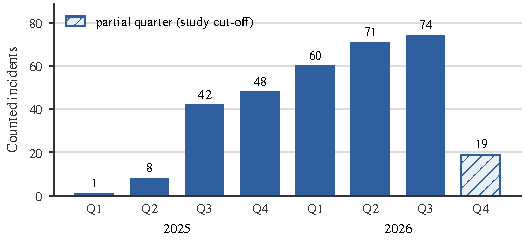
\includegraphics[width=0.85\columnwidth]{figures/rq3_timeline.pdf}
\caption{Verified harness incidents and CVEs by quarter of disclosure (RQ3). The final quarter is partial (to 15 October 2026) and does not indicate a decline.}
\label{fig:timeline}
\end{figure}

\paragraph*{Timeline} Disclosures rose in every complete quarter of the study period (Figure~\ref{fig:timeline}). The rise reflects more harnesses, greater researcher attention, wider use of GHSAs and an agent-assisted search that favours recent, well-indexed advisories, not necessarily declining quality; per-product counts likewise track scrutiny and disclosure maturity (D15) as much as risk, so we do not rank products by them.

\paragraph*{Root causes} Table~\ref{tab:rootcauses} gives the distribution. The largest group, with \nIncRCThree{} incidents (\pctRCThree{}), comprises defective checks that gate an agent capability (RC3): allowlists bypassed through shell substitution, redirection, environment-variable prefixes, \texttt{find -exec}, symlinks or look-alike domains. Configuration honoured before consent (RC2) contributes a further \nIncRCTwo{}: repository settings, hooks, \texttt{.env} files, MCP declarations and Git configuration that run or take effect before the trust prompt. Together these deterministic harness defects account for \pctRCTwoThree{} of counted incidents, the largest share though not a majority. Conventional defects not specific to agents (RC10) account for \pctRCTen{}, and missing authentication or Origin checks on local control endpoints (RC4) for \nIncRCFour{}. Pure prompt injection with no other control failure (RC1) stands at \pctRCOne{}; as the residual class, this is a lower bound on the role of injection, which we did not code separately as a vector.

\begin{table}[!t]
\centering\footnotesize
\caption{Root causes of the counted 2025--2026 harness incidents (RQ3), assigned by the ordered procedure. Primary taxonomy classes are given in Table~\ref{tab:taxonomy}.}
\label{tab:rootcauses}
\resizebox{\columnwidth}{!}{\begin{tabular}{lp{6.2cm}r}
\toprule
Root cause & Name & Incidents \\
\midrule
RC3 & Validation, parsing or authorization logic flaw in a check that gates an agent capability & 104 \\
RC2 & Workspace, repository or agent-written content executed or honoured before or without consent & 52 \\
RC10 & Conventional implementation defect not gating an agent capability & 51 \\
RC4 & Missing authentication or origin/Host validation on a local or network control endpoint & 24 \\
RC8 & Isolation boundary escape or weak isolation fallback & 20 \\
RC6 & Insecure default, missing safeguard or over-privileged mode by design & 20 \\
RC1 & Untrusted content treated as instructions (no distinct control failure) & 17 \\
RC7 & Unintended exposure, leakage or over-collection of secrets or data by the harness itself & 12 \\
RC5 & Package, extension or update-channel compromise or integrity failure & 11 \\
RC9 & Output-rendering or automatic-fetch feature acts as an exfiltration channel & 8 \\
RC12 & Adversarial use of a legitimate capability (no product defect) & 3 \\
RC11 & Autonomous action exceeding user intent without enforced guardrail & 1 \\
\bottomrule
\end{tabular}
}
\end{table}

\paragraph*{Classes} By primary class (Table~\ref{tab:taxonomy}), permission-model weaknesses (T03, \nIncTopThree{}, \pctTopThree{}) and repository configuration acting as code execution (T02, \nIncTopTwo{}) lead, followed by conventional defects (T19, \nIncTNineteen{}) and control-plane exposure (T18, \nIncTEighteen{}). Indirect prompt injection is the primary class of only \nIncTOne{} incidents, although injection is the delivery vector in many incidents classified elsewhere.

\paragraph*{Representative cases} Credit belongs to the original researchers. \emph{Injection to configuration:} hidden Unicode in rules files (Pillar Security)\evTP~\cite{pillar2025rulesfile}; injection flipping Copilot's auto-approve (CVE-2025-53773)\evTP~\cite{etr2025copilot}; Cursor executing attacker-written or silently modified MCP configuration (CVE-2025-54135/54136)\evD\evTP~\cite{cursor_54135,checkpoint2025mcpoison}. \emph{Configuration before consent:} Claude Code project files executing code and transmitting API tokens before the trust dialog (CVE-2025-59536, CVE-2026-21852)\evTP~\cite{checkpoint2026claude}; Codex CLI loading project MCP servers without confirmation (CVE-2025-61260)\evTP~\cite{checkpoint2025codex}; Gemini CLI's CI action auto-trusting the workspace\evD~\cite{ghsa_gemini_action}. \emph{Allowlist and path checks:} command deception in Gemini CLI\evTP~\cite{tracebit2025gemini}; path and command bypasses in Claude Code (CVE-2025-54794/54795)\evTP~\cite{cymulate2025inverse}, and deny rules not enforced through symlinks\evD~\cite{ghsa_cc_symlink}. \emph{MCP:} tool poisoning and the GitHub MCP leak (Invariant Labs)\evTP~\cite{invariant2025toolpoisoning,invariant2025github}; SQL-returned injection via the Supabase MCP server\evTP~\cite{generalanalysis2025supabase}; the unauthenticated proxy in MCP Inspector (CVE-2025-49596)\evD\evTP~\cite{mcp_inspector_49596,oligo2025inspector}. \emph{Other:} unauthenticated local control planes in OpenCode and DeepSeek Harness\evD~\cite{ghsa_opencode_server,ghsa_dsh_host}; a malicious prompt shipped in Amazon Q Developer 1.84.0\evD~\cite{amazonq2025}; the \texttt{nx} ``s1ngularity'' compromise, using installed AI CLIs to search for secrets\evD~\cite{nx2025s1ngularity}; data leaks from Antigravity shortly after launch\evTP~\cite{promptarmor2025antigravity,etr2025antigravity}; and a vendor's own account of the criminal misuse of a coding agent~\cite{anthropic2025aug}.

\paragraph*{Fix date relative to advisory publication} Among the \nLatency{} counted incidents with both dates, a fix release existed on or before the advisory's publication in \nLatencyBefore{} cases (median offset \nLatencyMedian{} days, maximum \nLatencyMax{}); \nIncNoFixDate{} incidents have no recorded fix date (unfixed or unknown). Because advisories are by design usually published after a fix, this measures disclosure practice rather than time to fix; report dates were not available.
